%------------------------------------------------------------------------------%
%                                                                              %
%                                                                              %
%   EnsiRapport Template                                                       %
%                                                                              %
%   Version : 1.0                                                              %
%                                                                              %
%   Auteur : Arthur Sonzogni                                                   %
%                                                                              %
%------------------------------------------------------------------------------%



\documentclass[liens,entete-ensimag,margeCorrection]{ensirapport}
% options possibles:
% -  ('10pt', '11pt' and '12pt') taille de police.
% -  ('a4paper', 'letterpaper', 'a5paper', 'legalpaper', 'executivepaper' and 'landscape') taille de papier.
% -  ('sans' and 'roman') famille de police.
% -- ('liens') ajoute les liens dans le sommaire.
% -- ('entete,entete-ensimag') ajoute des belles entetes avec logo ensimag ou pas.
% -- ('margeCorrection') diminue les enormes marges de latex.
% -- ('minted') inclus minted pour colorer les codes sources, ne fonctionne pas à l'ensimag.
% -  ('onecolumn','twocolumn') une ou deux colonnes
% -  ('fleqn','leqno') formules mathématique alignées a gauche ou a droite.
% -  ('notitlepage','titlepage') sans ou avec page de garde pour le titre

%\usepackage[draft]{graphicx}
\usepackage[nottoc, notlof, notlot]{tocbibind}
\setlength{\parindent}{0cm} % Défini la largeur de l'alinéa de 1cm.



\begin{document}


\title{Mon titre}
\author{Arthur Sonzogni}
\date{\today}

\renewcommand{\labelitemi}{\textbullet}

\large
\thispagestyle{plain}

\begin{center}


Institut National Polytechnique de Grenoble

École Nationale Supérieure d'Informatique et de Mathématiques Appliquées de
Grenoble

\vspace{0.4cm}


{\huge \bfseries HPC \& GPGPU}

\vspace{0.5cm}
{\large \bfseries Rapport des travaux}


\vspace{1.5cm}

\hrule width \textwidth height 2pt
\vspace{0.4cm}
{\Huge \bfseries HPC \& GPGPU.}
\vspace{0.4cm}
\hrule width \textwidth height 2pt

\vspace{2cm}

\end{center}
\begin{minipage}{0.5\textwidth}
    
{\it Auteurs:}

Arthur SONZOGNI
Thomas Coeffic

3A Grenoble INP - Ensimag

Filière MMIS (Modélisation Mathématique, Images, Simulation)

\end{minipage}


\vspace{2cm}

\begin{center}
Grenoble, le \today
\end{center}

\newpage
\normalsize

%\maketitle
\tableofcontents

\newpage

\section{Introduction}

L'idée que nous avons eut pour ces 2 projets et d'effectuer plusieurs versions du programme en utilisant différentes technologies et différentes approches.
Ceci nous permet d'effectuer des benchmarks intéressants.

\begin{enumerate}
    \item \textbf{Sequential}: programme de base non parallélisé.
    \item \textbf{HPC\_OpenMP}: parallélisation par groupes fixes d'agents (OpenMP)
    \item \textbf{HPC\_MPI}: Parallélisation par groupes fixes d'agents (MPI)
    \item \textbf{HPC\_MPI\_GRID}: Parallélisation spatiale : \\
                        groupes dynamique d'agents dans des cellules d'une grille.
    \item \textbf{GPGPU\_simple}: Parallélisation par groupes fixes d'agents (Cuda)
    \item \textbf{GPGPU\_Grid}: Parallélisation spatiale : 

\end{enumerate}


\section{Présentation des différents algorithmes}
\subsection{Sequential}

Pour chaques boids, on calcul sa nouvelle vitesse en fonction de l'ensemble des autres boids.
C'est cela qui donne une complexité quadratique au modèle.

On note n le nombre de boids :

\begin{align*}
    \text{Travail} &: O\left( n^2 \right)  \\
\end{align*}

\subsection{HPC\_OpenMP}
Le boucle principale parcours chaques agents pour déterminer sont incrément de vitesse.
L'algorithme se contente simplement de parallèliser cette boucle.

\begin{align*}
    \text{Travail} &: O\left( n^2 \right)  \\
    \text{Travail par processeur} &: O\left( \frac np \times n \right)  = O\left( \frac {n^2}p \right) \\
\end{align*}

Ainsi si $n\sim p$
\begin{align*}
    \text{Travail} &: O\left( n^2 \right)  \\
    \text{Travail par processeur} &: O\left( n \right) \\
\end{align*}

\subsection{HPC\_MPI}
Ici encore, on parallélise la boucle parcourant chaques agents.
Chaques processus à en charge une certaine proportion des boids.
Pour effectuer ces calculs il a besoin des positions et vitesse des boids géré par les autres processus.
Pour ce faire, après chaque tours, chaques processus effectue un envoie multicast de l'ensemble des boids dont il à la charge.

\begin{align*}
    \text{Travail} &: O\left( n^2 \right) \\
    \text{Travail par processeur} &: O\left( \frac n p \times n \right)  \\
    \text{Echange par processeur} &: O\left(n\right)
\end{align*}

Ainsi si $n \sim p$

\begin{align*}
    \text{Travail} &: O\left( n^2 \right) \\
    \text{Travail par processeur} &: O\left( n \right)  \\
    \text{Echange par processeur} &: O\left(n\right)
\end{align*}

\subsection{GPGPU\_Simple}

On effectue le même principe mais en utilisant la carte graphique.

\begin{align*}
    \text{Travail} &: O\left( n^2 \right) \\
    \text{Travail par cuda thread} &: O\left( \frac n p \times n \right)  \\
    \text{Accès mémoire globale} &: O\left(n\right)
\end{align*}

Ainsi si $n \sim p$

\begin{align*}
    \text{Travail} &: O\left( n^2 \right) \\
    \text{Travail par cuda thread} &: O\left( n \right)  \\
    \text{Accès mémoire globale} &: O\left(n\right)
\end{align*}

\subsection{HPC\_MPI\_GRID}

Pour cet algorithme, au lieu de subdiviser par rapport aux agents, on subdivise l'espace en une grille régulière de $n^3$ blocks.
On effectue les calculs des dépendances entre boids qui sont dans le même blocs.
On approxime l'influence des boids des blocs voisins comme la présence d'un gros boids virtuel de position et de vitesse représentant la moyennes du block
et de poids la somme des poids du bloc.

Une étape de l'algorithme se résume à :
\begin{itemize}
    \item Calcul du boids virtuel
    \item Envoie et réception des boids virtuel des voisins.
    \item Calcul de la nouvelle position et vitesse (influence des boids du bloc et des 6 boids virtuels voisins).
    \item Calcul des boids sortant.
    \item Envoie des boids sortant vers les blocs voinsin et réception des boids entrant.
\end{itemize}

Pour le calcul des complexité, on fera l'hypothèse que le nombre de boids par bloc reste suffisament constant.
Cette dernière n'est pas vraiment respecté en pratique et on peut voir des ralentissement lorsque qu'un trop gros groupe de boids se forme.

\begin{align*}
    \text{Travail} &: O\left( n^2 \right) \\
    \text{Travail par processeur} &: O\left( \left(\frac np \right)^2 \right)  \\
    \text{Echange par processeur} &: O\left( \left(\frac np \right)^2 \right)
\end{align*}

Ainsi si $n \sim p$

\begin{align*}
    \text{Travail} &: O\left( n^2 \right) \\
    \text{Travail par processeur} &: O\left( 1 \right)  \\
    \text{Echange par processeur} &: O\left( 1 \right)
\end{align*}

On a donc un système qui passe très bien à l'échelle. On ne communique qu'avec les 6 blocks voisins.
Le principale défaut est qu'on utilise l'approximation du boids virtuel.
La simulation est très rapidement différente que pour la simulation séquentiel, néanmoins, le comportement global est bien le même.

\subsection{GPGPU\_Grid}
On effectue le même principe mais en utilisant la carte graphique.

\textbf{TOTO explication}

\begin{align*}
    \text{Travail} &: O\left( n^2 \right) \\
    \text{Travail par cuda thread} &: O\left( \frac n p \times rc^2 \times n \right)  \\
    \text{Accès mémoire globale par thread} &: O\left( \frac n p \times rc^2 \times n \right)
\end{align*}

Ainsi si $n \sim p$

\begin{align*}
    \text{Travail} &: O\left( n^2 \right) \\
    \text{Travail par cuda thread} &: O\left( rc^2 \times n \right)  \\
    \text{Accès mémoire globale} &: O\left( rc^2 \times n \right)
\end{align*}

\section{Benchmarks}

Dans ce premier graphique nous souhaitons comparer globalement chaques algorithmes.

Nous ne faisons que varier le nombre d'agents.

Nous utilisons les machines de l'ensimag.


\begin{tabular}{|r|c|c|c|c|c|}
\hline
Nombre d'agents &Sequential  &HPC\_OpenMP  &HPC\_MPI\_GRID    &HPC\_GPU\_Simple  &HPC\_GPU\_GRID \\
\hline
1000&    4.71    &1.59    &5.88    &10.18   &6.70 \\
\hline
2000&    19.46   &6.40    &6.83    &21.37   &14.46 \\
\hline
3000&    42.15   &14.05   &14.00   &32.83   &22.62 \\
\hline
4000&    71.86   &24.63   &17.45   &45.66   &31.10 \\
\hline
5000&    111.412 &37.926  &24.214  &58.947  &44.251 \\
\hline
6000&    162.402 &55.542  &30.664  &70.334  &58.64 \\
\hline
7000&    226.902 &76.452  &40.654  &86.295  &75.249 \\
\hline
\end{tabular}

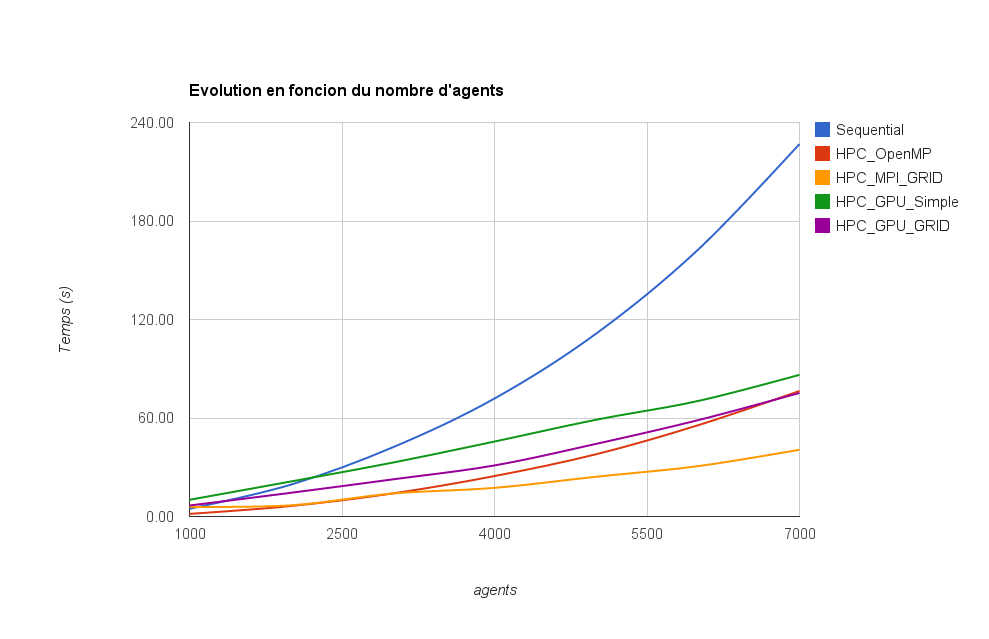
\includegraphics[width=\linewidth]{imageGlobale}

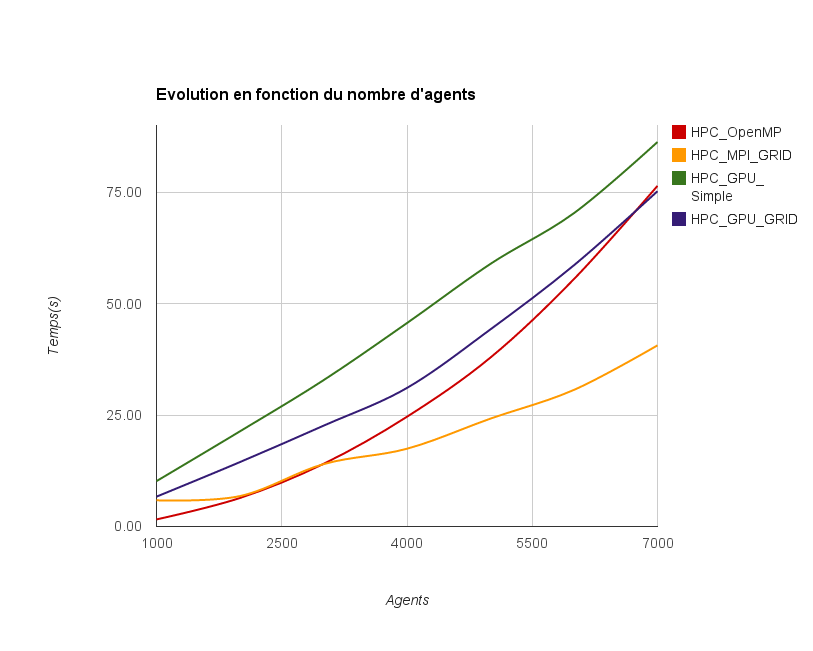
\includegraphics[width=\linewidth]{imageGlobalLight}

\end{document}

